\documentclass[a4paper, 12pt]{article}
\usepackage[utf8]{inputenc}
\usepackage[english,russian]{babel}
\usepackage[warn]{mathtext}
\usepackage{graphicx}
\usepackage{float}
\restylefloat{table}
\usepackage{amsmath}
\usepackage{floatflt}
\usepackage[T2A]{fontenc}
\usepackage[left=20mm, top=20mm, right=20mm, bottom=20mm, footskip=10mm]{geometry}

\tolerance 1414
\hbadness 1414
\emergencystretch 1.5em
\hfuzz 0.3pt        % размер максимального переполнения без warning'a
\widowpenalty=10000 % запрещает одиночную строку абзаца в начале страницы
\vfuzz \hfuzz
\raggedbottom       % если на странице мало содержимого, добавить пустое место в конце, а не в середине страницы



\begin{document}

\begin{titlepage}
	\centering
	\vspace{5cm}
	{\scshape\LARGE московский физико-технический институт (национальный исследовательский университет) \par}
	\vspace{6cm}
	{\scshape\Large Лабораторная работа 3.3.3\par}
	{\huge\bfseries Опыт Милликена \par}
	\vspace{1cm}
	\vfill
\begin{flushright}
	{\large Б03-102}\par
	\vspace{0.3cm}
	{\LARGE Куланов Александр}
\end{flushright}
	

	\vfill


	Долгопрудный, 2022 г.
\end{titlepage}

\begin{itemize}
	\item \textbf{Цель работы:} измерение элементарного заряда
    \item \textbf{В работе используются:} плоский конденсатор в защитном кожухе, измерительный микроскоп, электростатический вольтметр,
    секундомер, переключатель напряжений, пульверизатор с маслом
    
\end{itemize}

\section{Теоретические сведения}

Если элементарный заряд существует, то все заряды будут ему кратны. В опыте будут измерятся заряды капелек масла, несущих несколько элементарных зарядов.

Для измерения заряда будем исследовать движение капелек в электрическом поле. Уравнение движения капли при свободном падении
\begin{equation}
m \dfrac{dv}{dt}=mg-F_{\text{тр}},
\end{equation}
где $m$ -- масса капли, $v$ -- её скорость, $F_{\text{тр}}=6\pi \eta rv = kv$ -- сила вязкого трения, $r$ -- радиус капли, $\eta$ -- коэффициент вязкости воздуха. Отсюда получаем 
\begin{equation}
v = \dfrac{mg}{k}\left(1 - e^{-kt/m}\right).
\end{equation}
Скорость установится на
$$
v_{\text{уст}}=\dfrac{mg}{k}=\dfrac{2}{9}\dfrac{\rho}{\eta}gr^2,
$$
где $\rho$ -- плотность масла. Установление этой скорости происходит с постоянной
$$
\tau = \dfrac{m}{k}=\dfrac{2}{9}\dfrac{\rho}{\eta}r^2
$$
Обозначая $h$ путь капли, пройденный за $t_0$, получаем формулу для её радуса:
\begin{equation}
r = \sqrt{\dfrac{9\eta h}{2\rho gt_0}}.
\end{equation}
В случае движения в электрическом поле конденсатора с разностью потенциалов $V$ и расстоянием $l$ между пластинами получаем уравнение движения
\begin{equation}
m \dfrac{dv}{dt}=\dfrac{qV}{l}-mg-kv,
\end{equation}
Новое слагаемое не влияет на $\tau$, новая установившаяся скорость
$$
v_{\text{уст}}'=\dfrac{qV/l - mg}{k}.
$$
Если $t$ -- время подъёма на высоту $h$, то можно получить формулу заряда капли:
$$
\dfrac{qV}{kl}-v_{\text{уст}}=v_{\text{уси}}'=\dfrac{h}{t};
$$
$$
k=6\pi \eta r  = 6\pi \eta  \sqrt{\dfrac{9\eta h}{2\rho gt_0}};
$$
\begin{center}
$\Rightarrow$ \fbox{$q = 9\pi \sqrt{\dfrac{2\eta^3 h^3}{g\rho}}\cdot \dfrac{l(t_0+t)}{Vt^{3/2}_0t}$}
\end{center}

\section{Экспериментальная установка}

\begin{figure}[H]
    \centering
    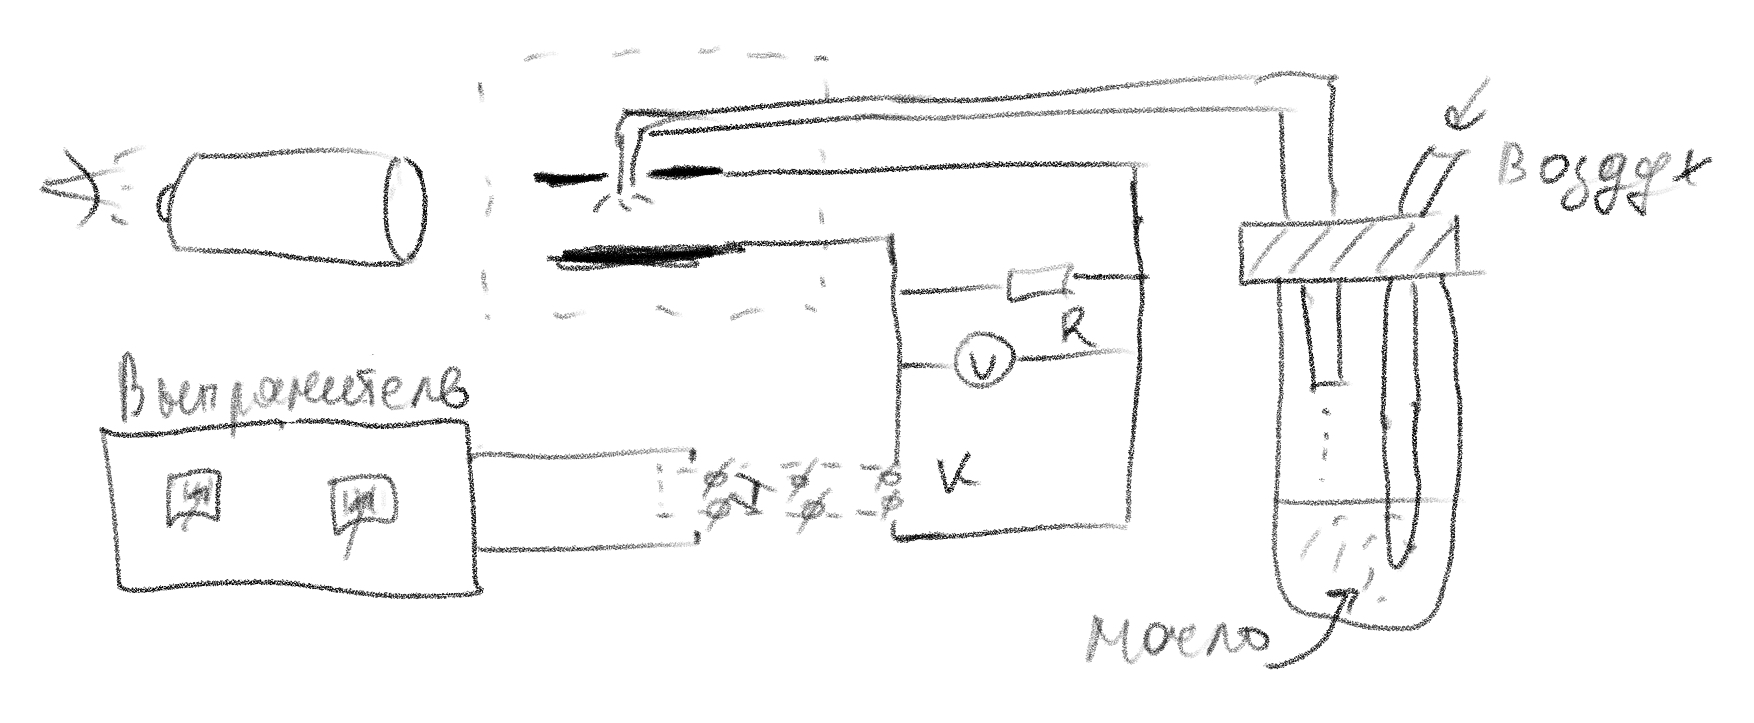
\includegraphics[width=1\textwidth]{set}
    \caption{Схема установки}
    \label{fig:set}
\end{figure}

Схема преставлена на рисунке \ref{fig:set}. Масло разбрызгивается пульверизатором, попадает на конденсатор $C$ через небольное отверстие, приобретая заряд засчёт трения о воздух.
Напряжение подаётся с выпрямителя и измеряется вольтметром $V$. Ключ $K$ позволяет менять направление поля кондексатора. При замыкании конденсатор разряжается в $R \approx 10~\text{МОм}$.
Для наблюдения за каплями установлен микроскоп, в фокальной плоскости окуляра которого  виден ряд горизонтальных линий с предварительно определённым расстоянием между ними. Время движения капель замеряется электронным секундомером.



\section{Обработка результатов}



\section{Приложение}



\end{document}